We have implemented our approach in \whoop, a prototype infrastructure that combines static lockset analysis with state-of-the-art compilation and sequential verification techniques to (i) soundly analyse Linux kernel modules for data races and (ii) accelerate a plugged-in bug finder.

\begin{figure*}
\centering
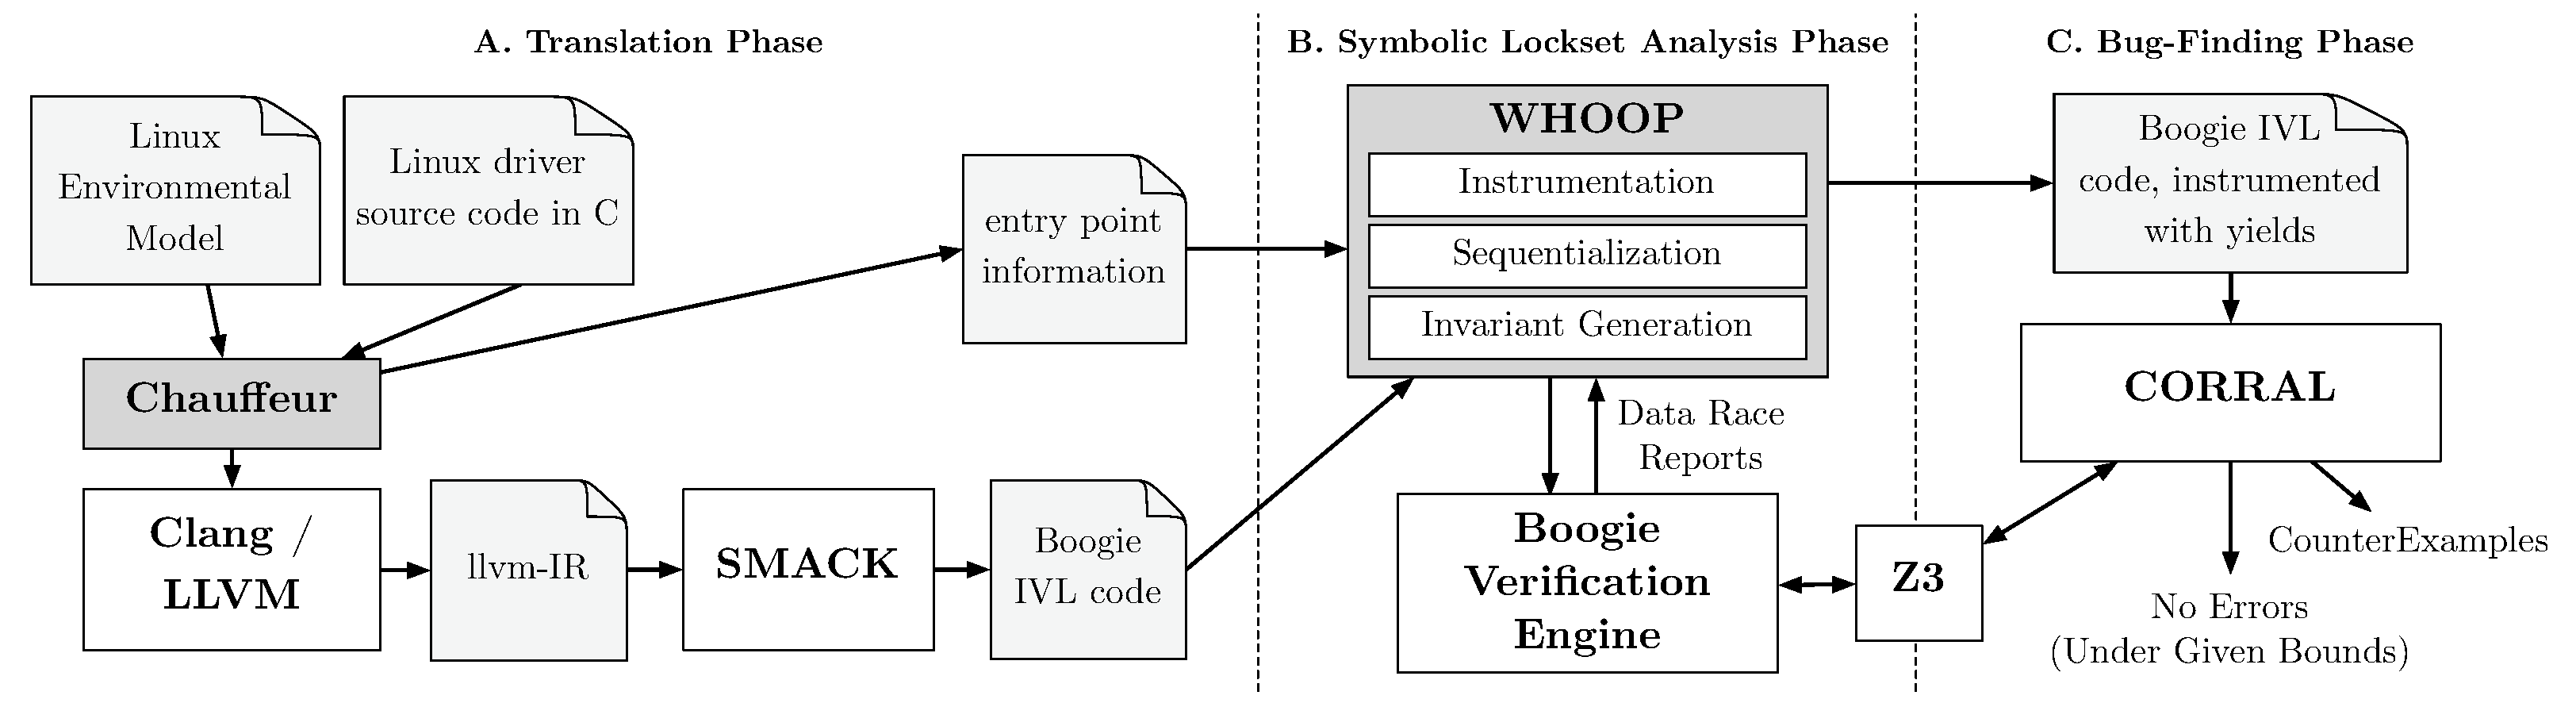
\includegraphics[width=.99\linewidth]{img/whoop.pdf}
\caption{The \whoop infrastructure, empowered by state-of-the-art compilation (Clang/LLVM and SMACK) and verification (Boogie and \corral) tools}
\label{fig:whoop}
\end{figure*}

Figure~\ref{fig:whoop} depicts the \whoop infrastructure. Initially, \whoop accepts a kernel module written in C, together with a Linux environmental model. The environmental model (i.e. stub Linux header files) is required to ``close'' the module and allow it to be translated and subsequently analysed. Both the module and the environmental model are passed to the translation phase of \whoop (see Section~\ref{translation}), which outputs an over-approximated program written in the Boogie intermediate verification language (IVL)~\cite{deline2005boogiepl}. Next, \whoop performs its static lockset analysis (see Section~\ref{staticanalysis}) to detect all potential data races in the abstract program. Finally, \whoop uses information from the static analysis phase to accelerate bug finding with \corral (see Section~\ref{bugfinding}).